\section{Introduction}

From report

During the last quarter the team from Indiana focused on additional statistical analyses to identify scientific impact metrics that would correlate with use of XSEDE resources.  This was carried out by extending previous work, and introducing additional correlations to other relevant data sets, including resource allocation data from TeraGrid/XSEDE, and institutional data curated by Clemson University (see for example Amy Apon: High Performance Computing Instrumentation and Research Productivity in U.S. Universities, Journal of Information Technology Impact, Vol. 10, No. 2, pp. 87-98, 2010).

With respect to XSEDE allocations, to date we have found no obvious correlation between the scientific impact and the individual project level, which is the base unit on which resource allocations are granted.  However, we did find a trend correlating the allocations made to different Fields of Science (FOS), see Figure 3.3-1. This figure depicts that the overall scientific impact metrics of one FOS is significantly correlated to the resource allocation for the projects in that FOS. 
 
Figure 3.3-1 Correlation between field of science and XSEDE allocation. The dot size is proportional to number of projects in that FOS.

To better mine the data, we have created a simple Web portal allowing to interactively look at the data. The screenshot of this Web portal (http://fgdev.pti.indiana.edu:8088/fosvsalloc) is shown in Figure 3.3-2.  The upper plot shows the name, impact metric, and allocation data for a FOS.  The bottom figure is produced by removing the trend and thus helps to emphasize how the FOS diverges from the trend. 

Figure 3.3-2: The portal provides the ability to reveal the specific data while hovering over a field of science entry point, making it convenient for interactive data exploration.  The top plot shows the correlation between allocations and publications (h-index).  The bottom plot shows the FOS impact when the data have been detrended.

Hence we can make the following observations:

\begin{enumerate}

\item We find that several FOS with the similar h-index use fewer resources than others showing better relative output measured by the h-index. This is done by comparing FOS on a vertical slice of the h-index (see Figure 3.3-3). 
 
Figure 3.3-3: Interactively comparing projects with similar h-index 

\item The trend introduces a baseline of 0. FOS above 0 use more resources than the trend, FOS bellow 0 use less resources to produce the expected impact based on a given h-index.

From Figure 3.3-1 we can deduct that the more projects are in a FOS the greater the impact is. 

\item We have found some outliers that we want to investigate in the next quarter more carefully (see Figure 3.3-4).

\item We can roughly categorize the projects into four classes which will help in categorizing the projects more easily by h-index (see Figure 3.3-4).
 
Figure 3.3-4: Rough classification of FOS by h-index

\item Based on these and other observations, we are working on an allocation-index or a-index that takes the h-index and allocations to produce a single comparative measurement.

\end{enumerate}

We anticipate that the results will be  integrated directly into XDMOD framework so the XSEDE administrative and/or XRAC committee will have a single entry point to get the relevant information. 

Additional work is warranted while identifying and potentially integrating other datasets such as the data from Clemson University. This would help us to identify other causes and correlation than the actual allocation sizes. Together the metrics will be useful both in serving as an auditing tool for XSEDE resource allocation, and in giving reference and guidance about which Fields of Science results in more scientific output measured by for example the h-index.  It is important to track this information over long periods of time as to for example identify if more allocations to a project or FOS result in more publications.

We have obtained institutional specific data maintained by Dr. Amy
Apon at Clemson University, and carried out preliminary analysis by
correlating that data with our metrics data. The institutional data
set consists of a list of US research institutions that are classified
as having very high research activity or high research activity by
Carnegie Foundation \cite{carnegiefoundation-decription}. For each institution, the yearly publication count data are available from year 2005 to year 2009. For the correlation analysis, we aggregated the publications we have collected also in organization level, and compared the publication counts from the same institutions from 2005 to 2009. From the preliminary results we see that for most institutions in the list, while the annual number of publications grew steadily, the number from users that were related to TeraGrid/XSEDE grew even more rapidly. Furthermore, as shown in Figure 3.3-5 the distribution and median (indicated by a blue line) year over year (YOY) growth rate of the percentage (of TG/XD pubs/ALL pubs for an institution), it was increasing for all the YOY comparisons, while the increasing rate was slowing down.

 
Figure 3.3-5: Year over Year growth rate of TG/XD users’ publications’ share of all the publications for each institution. A red line indicates where a zero growth is supposed to be, and a blue line shows the median growth rate from all the institutions.
The result could be interpreted as that either TG/XD attracted more users along the years or the users produced more publications or both, however as we are lacking some supporting data here, we cannot reach a definite conclusion. We will be further exploring the data and solidifying the preliminary result while trying to find and integrate with other data sets from XSEDE and other sources.

Furthermore, we worked on improving our software system including both additional data and the upgraded services. Our framework is simple but carefully designed to not only integrate into the TAS portal, but also the XSEDE portal as requested by Maytal Dahan from TACC and the POPS systems that is under redesign. The underlying infrastructure is independent but as the same software tools are used as in TAS they can be easily integrated. The development portal we use is needed for developing quick views that can later be integrated into the TAS and XSEDE portals. This has greatly increased our productivity, while also being able to show some of our results in an interactive fashion to users and sponsors. It allows us also to discuss ideas with other groups quickly such as the interaction with Clemson University and TACC have proven. The overall work to produce our portal framework was small, as we leveraged the portal framework used in FutureGrid to interact with cloud metric systems (less than one week total). This could also provide a potential pathway forward to expose cloud metric data to XSEDE if it were to become relevant.

\begin{figure}[htb]
  \centering
    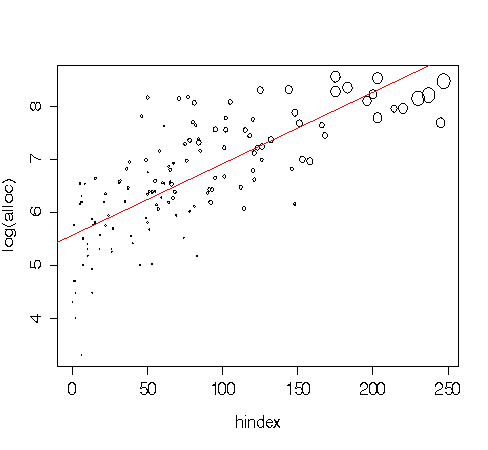
\includegraphics[width=1.0\columnwidth]{images/fig1.pdf}
  \caption{fig1.}\label{F:fig1}
\end{figure}

\begin{figure}[htb]
  \centering
    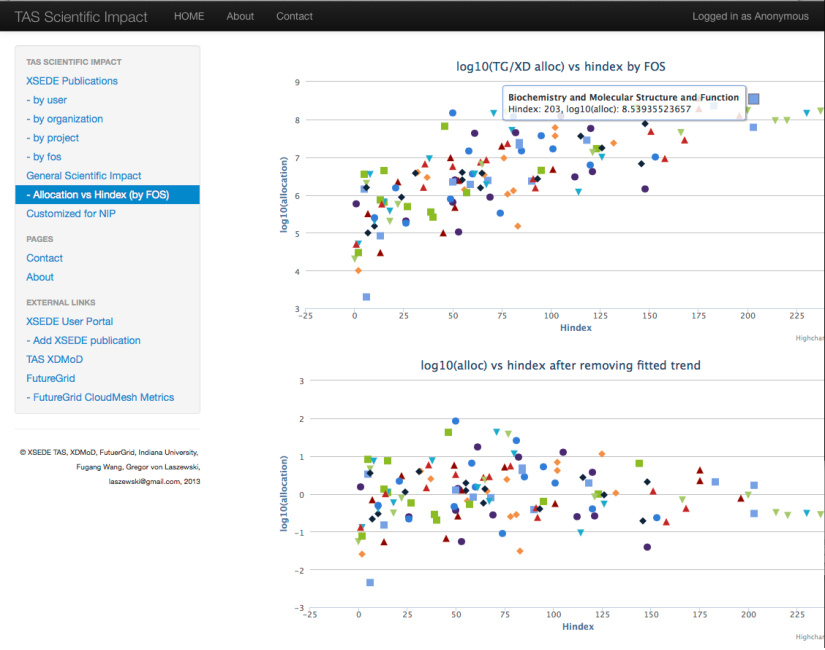
\includegraphics[width=1.0\columnwidth]{images/fig2.pdf}
  \caption{fig2.}\label{F:fig2}
\end{figure}

\begin{figure}[htb]
  \centering
    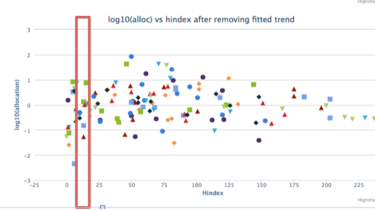
\includegraphics[width=1.0\columnwidth]{images/fig3.pdf}
  \caption{fig3.}\label{F:fig3}
\end{figure}

\begin{figure}[htb]
  \centering
    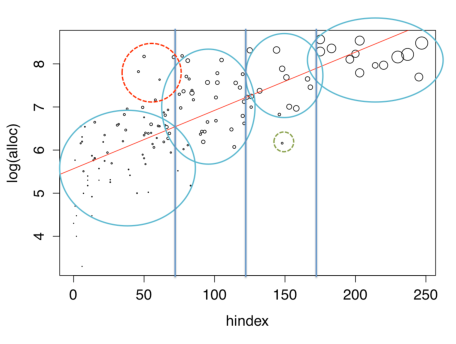
\includegraphics[width=1.0\columnwidth]{images/fig4.pdf}
  \caption{fig4.}\label{F:fig4}
\end{figure}

\begin{figure*}[htb]
  \centering
    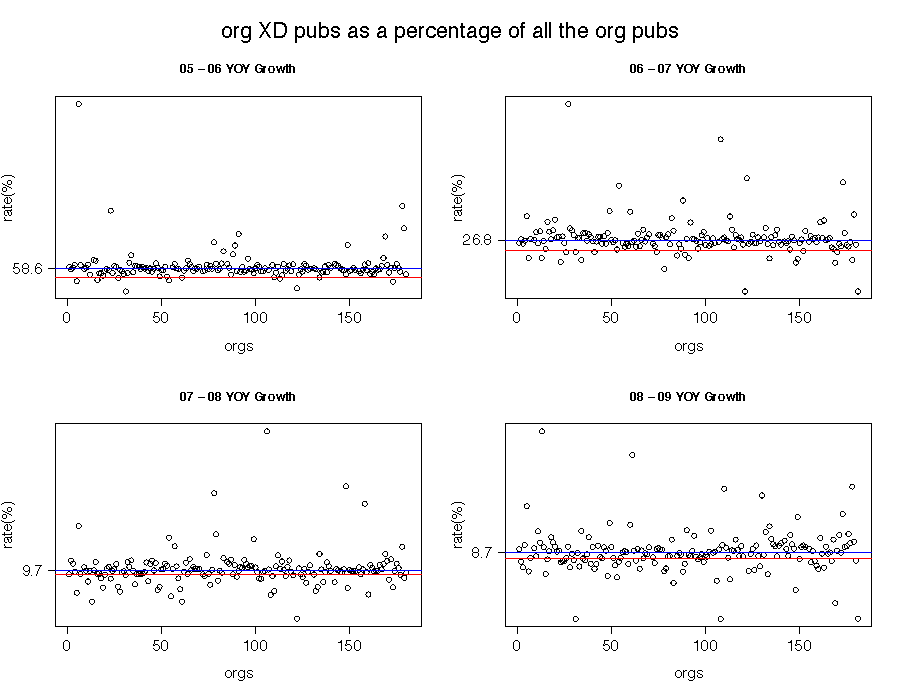
\includegraphics[width=1.0\textwidth]{images/fig5.pdf}
  \caption{fig5.}\label{F:fig5}
\end{figure*}

